\begin{frame}{RTV: varias revisiones, un estado común}
  \vspace{-0.15cm}
  {\footnotesize García Sangoquiza \textbullet{} Giraldo Cagua \textbullet{}
  Herrera Barco \textbullet{} Lombeida Escaleras\par}
  \vspace{0.12cm}
  \begin{columns}[T,onlytextwidth]
    \begin{column}{0.61\textwidth}
      \begin{block}{Centro de revisión de Valencia}
        \small Gestiona turnos, pruebas y certificados.\\[0.12cm]
        Recepción, recaudación, inspectores y jefatura.
      \end{block}
    \end{column}
    \begin{column}{0.35\textwidth}
      \begin{block}{Alcance documentado}
        {\Large\bfseries 1 centro municipal}\\[0.10cm]
        \small Varias líneas: requisito RNF-08.\\
        {\scriptsize No hay carga real medida.}
      \end{block}
    \end{column}
  \end{columns}
  \vspace{0.08cm}
  {\small
  \textbf{Paralelismo:} ejecutar tareas al mismo tiempo.\\[0.10cm]
  \textbf{Distribución:} componentes que cooperan por red.\\[0.10cm]
  \textbf{En RTV:} concurrencia entre revisiones; CPU no verificada.\par}
  \vfill
  {\scriptsize Caso académico: backend y BD en nodos separados, por supuesto explícito.\par
  Fuentes: \cite{gs_rtv,gs_oracle_hilos}.}
\end{frame}

\begin{frame}{Arquitectura: quién coordina y dónde está el estado}
  \vspace{-0.12cm}
  \centering
  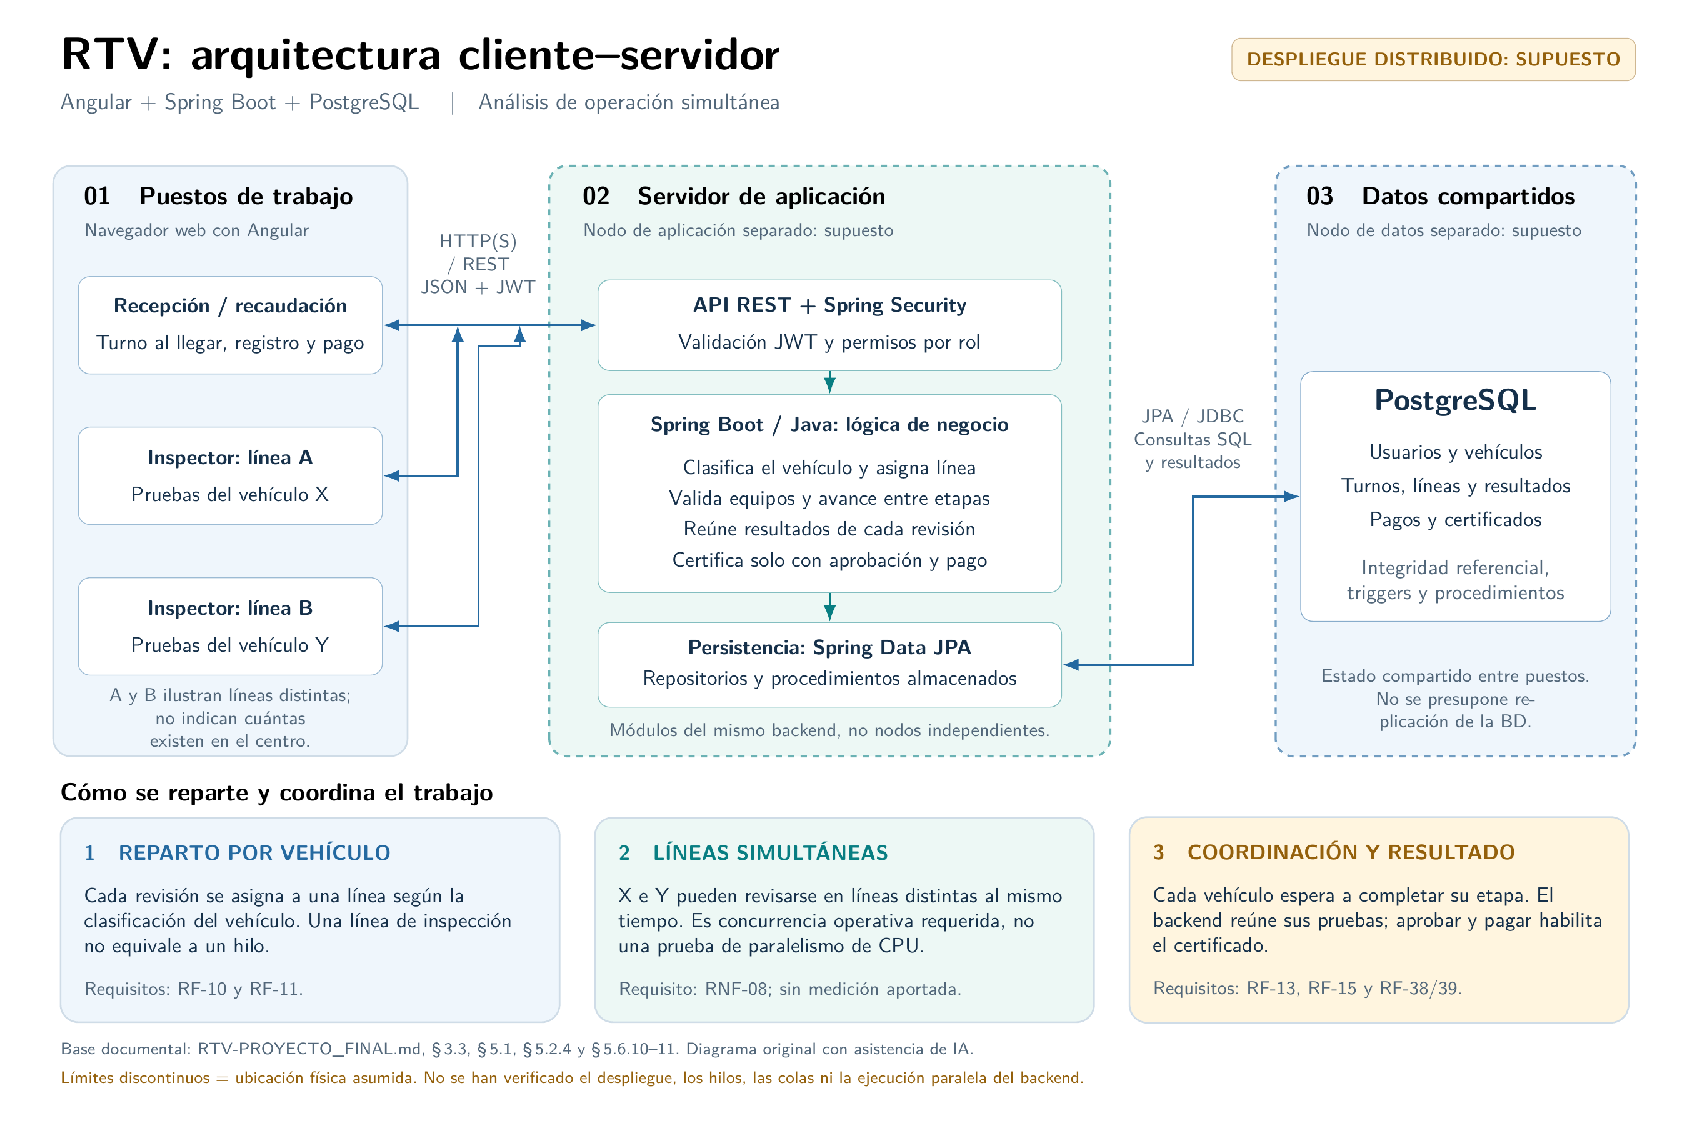
\includegraphics[width=\textwidth,height=4.35cm,keepaspectratio]{figuras/gs_arquitectura_resumen.pdf}
  \par\vspace{0.08cm}
  \raggedright
  {\small \textbf{Reparto:} por vehículo y línea. \quad
  \textbf{Reunión:} resultados de cada revisión.\par}
  \vspace{0.10cm}
  {\scriptsize Límites discontinuos: nodos físicos asumidos, no despliegue comprobado.\\
  Los módulos del backend no son microservicios. Un puesto no equivale a un hilo.\\
  Fuentes: documento RTV, \S\,3.3 y RF-10/11/15 \cite{gs_rtv};
  vocabulario REST: \cite{gs_spring_servlet}.}
\end{frame}

\begin{frame}{Dos revisiones concurrentes; cada una avanza en orden}
  \vspace{-0.10cm}
  \centering
  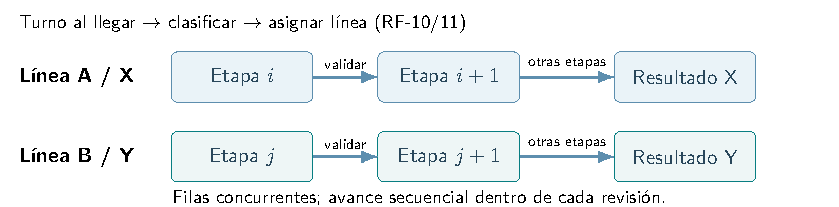
\includegraphics[width=\textwidth,height=3.2cm,keepaspectratio]{figuras/gs_recorrido.pdf}
  \par\vspace{0.05cm}
  \raggedright
  \begin{columns}[T,onlytextwidth]
    \begin{column}{0.49\textwidth}
      \begin{block}{Qué debe esperar}
        \small Etapa completa + equipo válido.\\
        Certificado: aprobado \textbf{y} pagado.
      \end{block}
    \end{column}
    \begin{column}{0.47\textwidth}
      \begin{block}{Qué no se ha demostrado}
        \small Hilos, aceleración o correo asíncrono.\\
        MVCC no sustituye las reglas del negocio.
      \end{block}
    \end{column}
  \end{columns}
  \vfill
  {\scriptsize Ejemplo ilustrativo: A/B y X/Y no son cifras de operación. Etapas genéricas, no tiempos reales.\\
  Fuentes: RNF-08, RF-13/24/25/38/39 \cite{gs_rtv}; MVCC \cite{gs_postgresql17}.}
\end{frame}
